%\documentclass[10pt,conference]{IEEEtran}
% If the IEEEtran.cls has not been installed into the LaTeX system files,
% manually specify the path to it:
\documentclass[letterpaper,10pt,conference]{/home/pranav/Desktop/Publication_work/latex_class_files/IEEEtran}
\usepackage{geometry}
\usepackage[]{amsmath}
\usepackage[pdftex]{graphicx}
\usepackage{url}
\usepackage{subfig}
\usepackage{tabularx}


\begin{document}

% paper title
\title{Achieving Seamlessness in Multi-Projector based Tiled Display using Camera Feedback}


% author names and affiliations
% use a multiple column layout for up to three different
% affiliations



\author{
    \IEEEauthorblockN{Pranav Kant Gaur\IEEEauthorrefmark{1}, Dinesh M. Sarode\IEEEauthorrefmark{1}, Pritam P. Shete\IEEEauthorrefmark{1}, Venkata P.P.K\IEEEauthorrefmark{1}, S.K. Bose\IEEEauthorrefmark{1}}
    \IEEEauthorblockA{\IEEEauthorrefmark{1}Computer Division, Bhabha Atomic Research Centre
    \\\{pranav,dinesh,ppshete,panikv,bose\}@barc.gov.in}
}



    



\maketitle

\begin{abstract}
High resolution displays utilizing an array of commodity projectors are becoming popular approach(also called \textit{tiled displays}) for visualizing high resolution content like scientific data-sets. These systems provide a relatively cheaper and flexible alternative to displays based on single high resolution monitor or projector. This approach inherently provides a method to create displays with resolution much higher than that possible by using a single high resolution display device. However, bezels in monitor based tiled displays obstruct the geometric continuity of the rendered content. In this paper, we describe the algorithms for geometric alignment of projection regions of an array of arbitrarily placed projectors and attenuation of projected intensities in the overlapping regions of multiple projectors using camera as a feedback device. Combination of these algorithms help us achieve a seamless high resolution display. We have observed improvements in fidelity of the rendered content by utilizing \textit{collinearity} constraint in geometric alignment calculations. We also propose a novel technique based on \textit{cross-ratio} invariant for utilizing full projection region of individual projectors which was limited by the size of features used for geometric alignment in the earlier approaches for planar displays. This also results in more imperceptible edge blending artifacts for same physical setup of projectors.
\end{abstract}

\begin{IEEEkeywords}
geometric alignment, edge blending, collinearity, cross-ratio, multi-projector display
\end{IEEEkeywords}

\section{Introduction}
Tiled displays provide an alternative to the visualization of high resolution content over single large scale high resolution monitor(or projector) by attaining comparable performance using combination of low cost and low resolution commodity displays. Tiled displays have been realized either using grid of monitors\cite{bose,harish} or projectors\cite{brown,judson,raskar,majum}. Using LCD monitors provides a compact, relatively cheaper and readily configurable high resolution visualization solution, though it still cannot completely imitate a single high resolution display because bezels of monitors obstruct the geometric continuity of the rendered content. Whereas in a multiprojector system, projectors may be arbitrarily placed and they inherently do not enforce any limitations of physical seams. Our work addresses \textit{seamless} rendering of the content using projectors. \par
Projectors will have quad shaped projection region without necessarily ensuring geometric continuity over the projected content. Manual \textit{keystoning} to geometrically align content from multiple projectors on the screen is time consuming and tedious. Further, it can easily become impractical for large number of projectors. Brown's\cite{brown} approach relaxes that assumption and instead allows for a casual positioning of projectors. It aims to create geometrically seamless and rectangular image in camera-space which guarantees geometrical seamlessness on the screen. But it does not guarantee rectangular output on the screen. Further, the usable projection region is limited by the size of features used for geometric alignment. Our contribution through this work is to remove the above mentioned limitations in \cite{brown} for the case when projection screen is planar. Further, by utilizing the \textit{collinearity} constraint in geometric alignment calculations we have observed more accurate final rendering.\par



\section{Solution overview}
We assume an ideal arrangement where all projectors are identical, the principle axes of each projector is orthogonal to the display screen and all are at equal perpendicular distance from the screen. In such an arrangement, we only need to partition the image and assign individual partitions(or rectangular \textit{tiles}) to each projector to get \textit{geometrically continous} projection of the content on the screen. Effectively, it emulates a single high resolution display.\newline
However, in a practical setup of array of projectors, they are not necessarily identical. Further, they may be arbitrarily positioned and oriented. In this case, the projection on the screen and corresponding image in the projector frame buffer may not be uniformly scaled forms of each other but will depend upon the projector orientation and its position with respect to projection screen. Precisely, the projection region of each projector will be a quad unlike the rectangular one in case of the above mentioned ideal arrangement.\newline
Therefore, to transform this arrangement back to our ideal configuration(without any physical manipulation) we need to determine the the \textit{tile configuration}. The tile configuration for a multiprojector display describes the share of each projector(or the \textit{tile}) in the image to be projected. Further, we also need to determine the distortion we should introduce in each tile so that when projected it remain geometrically continous with the content projected by adjacent projectors.\newline
To observe such deviations of physical configuration of projectors with respect to the ideal configuration, we use a camera as a feedback device and a reference pattern is projected by each projector. For each projector, camera records the distortion of this reference pattern with respect to ideal projection discussed above. Based on the boundaries of each projection region(called the \textit{bounding box} in camera image), we determine the share of each projector in the image(or the \textit{tile configuration}). Using the distortion information of the reference pattern captured by camera(for each projector) with respect to the image in the projector frame buffer we determine a distortion map called the \textit{warp map}. Finally, system gives geometrically continous content by distorting each \textit{tile} using the \textit{warp map}.\newline 
Further, the adjacent projectors may have overlap in their projection regions resulting in brighter regions at their boundaries, therefore it is necessary to attenuate(or \textit{edge blend}) the intensity of projected images in such regions so that overall projected content appears \textit{seamless}. Figure \ref{setup} shows our display screen with 3X3 rear-projection projector array and rendering cluster driving the display. We place camera in front of the projection screen to capture the projected reference patterns.
\begin{figure}
\centering
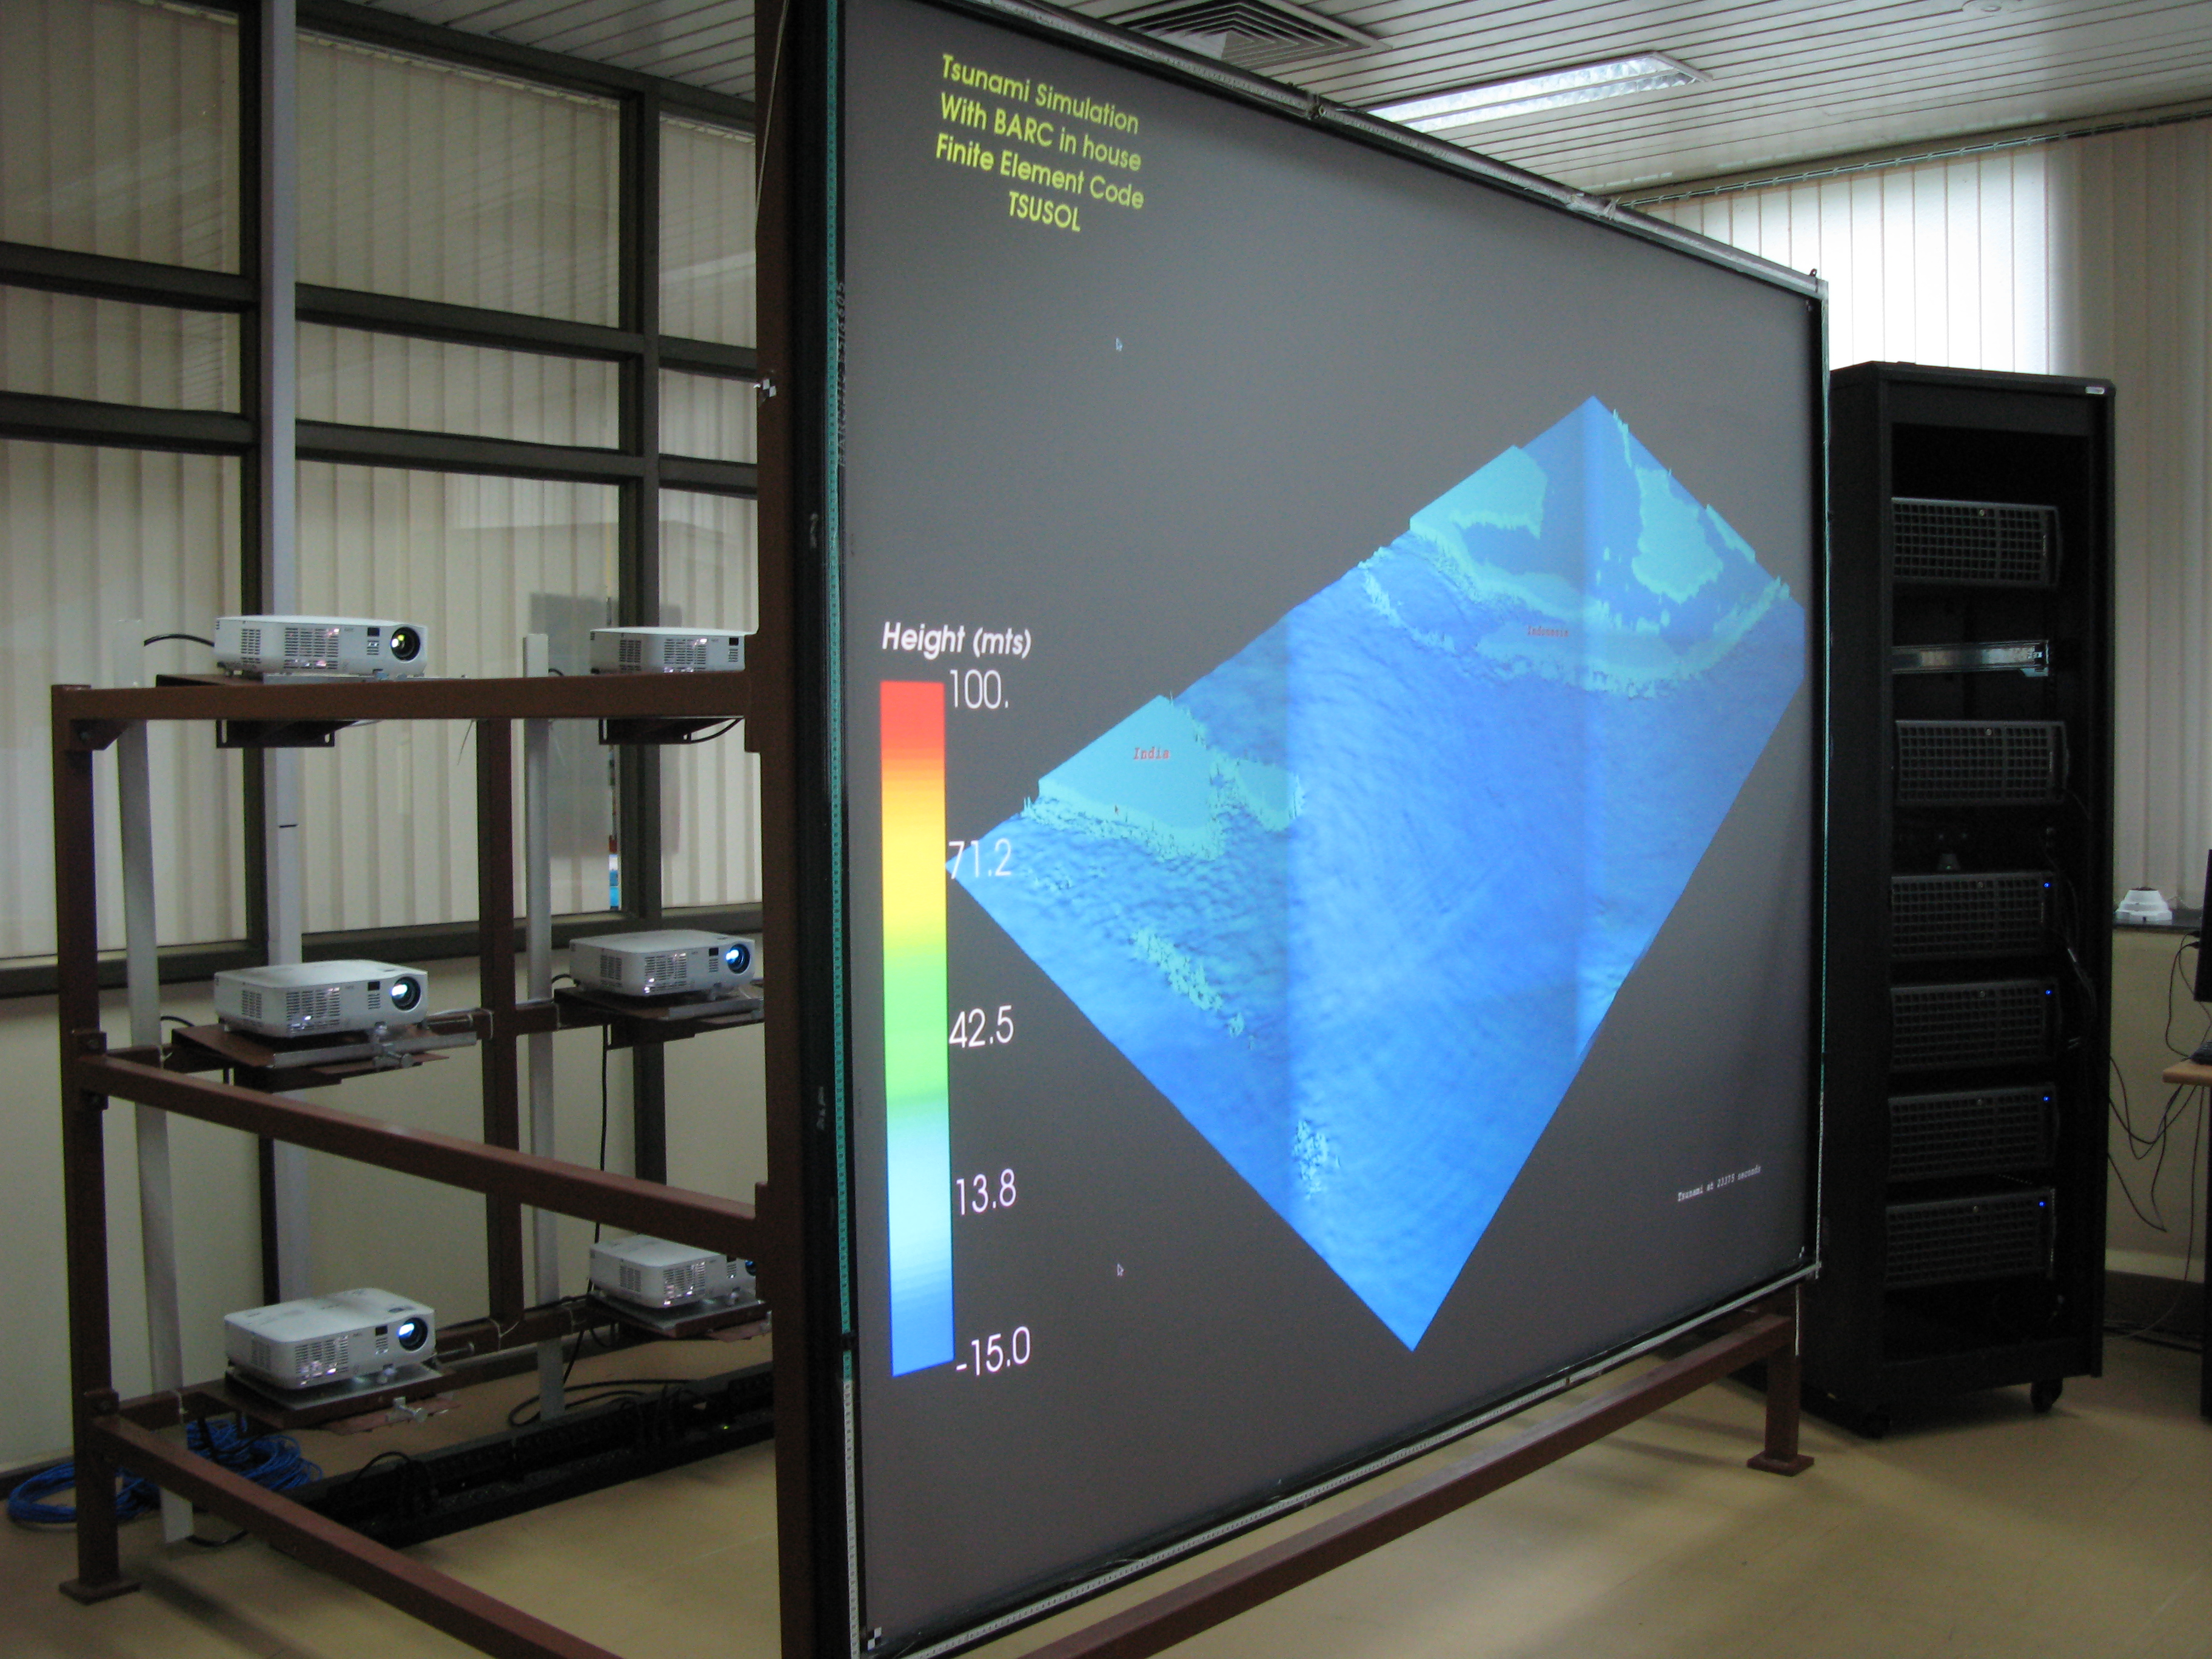
\includegraphics[width=6cm,height=4cm]{figures/system_setup.jpg}
\caption{Our 3X3 multiprojector display system}
\label{setup}
\end{figure}



\section{Geometric alignment}
Geometric alignment in \cite{brown} limits the usable projection region of each projector to the region within the quad of the outermost features used for geometric alignment. In this work, we propose to utilize \textit{cross-ratio}\cite{hartley} invariance which is preserved between perspective projection from projector to planar screen and planar screen to camera in order to recover entire projection region of individual projectors. It also eliminates another implicit limitation of \cite{brown} which requires adjacent projectors to atleast have overlap among the outermost features of their reference patterns on the screen, this limits the flexibility of positioning of individual projectors. 


\subsection{Cross-ratio invariance}
Assuming planer perspective projection of features from the projector to screen and from the screen to camera, we can recover coordinates of an unknown point(say 'A') in camera image given the coordinates of other three(i.e.,'B','C','D' are known) using cross-ratio invariant. Let $A_p$,$B_p$,$C_p$,$D_p$ be the coordinates of 4 collinear points in projector space and $A_c$,$B_c$,$C_c$,$D_c$ be the corresponding projection in camera space. Here, $B_c$,$C_c$ and $D_c$ are known whereas $A_c$ is unknown but $A_p$,$B_p$,$C_p$,$D_p$ are all known. Let us further represent the line joining $A_c$,$B_c$,$C_c$,$D_c$ in parametric form as:
\begin{equation}
\begin{aligned}
x_t=B_c^x+t*(D_c^x-B_c^x)\\
y_t=B_c^y+t*(D_c^y-B_c^y)
\end{aligned}
\label{paramet}
\end{equation}
where, $(x_t,y_t)$ are parametric coordinates of an unknown point(in our case $A_c$)\newline
Utilizing cross-ratio invariance yields following relation:
\begin{equation}
CR_p=\frac{|AC|_c*|BD|_c}{|BC|_c*|AD|_c}
\label{cross_rat_eqn}
\end{equation}
Here $CR_p$ is the cross-ratio computed in projector-space, $|ab|_c$ represents Euclidean distance between points $a$ and $b$ in camera-space. Using equation \ref{cross_rat_eqn}, we get quadratic equation with following possible solutions:
\begin{equation}
[t_1,t_2]=\frac{-b\pm\sqrt{b^{2}-4ac}}{2a}\\
\label{quad_eqn}
\end{equation}
where,\newline
Let,\newline
$delta={CR_p*(\frac{|BC|_c}{|BD|_c})}^2$\newline
Then,
\newline
$a=(1-delta)*|BD|_c^2$\newline
\begin{eqnarray*}
b=2*{(D_c^x-B_c^x)*(B_c^x-C_c^x)+(D_c^y-B_c^y)*\\(B_c^y-C_c^y)} + 2*|BD|_c^{2}*delta
\end{eqnarray*}
$c=|BC|_c^2-delta*|BD|_c^2$ \newline

Based on the convention of the chosen coordinate system, only one of $t_1$ or $t_2$ will be the valid position of the unknown point $A_c$. Figure \ref{cross_rat_img} shows a close view of a projected checkerboard(used as \textit{reference pattern} in our work) in camera image. Specifically, in figure \ref{cross_rat_img} an unknown point $A_c$ collinear with $B_c$,$C_c$,$D_c$ can be recovered by utilizing equation \ref{paramet}. 

\begin{figure}[ht]
\centering
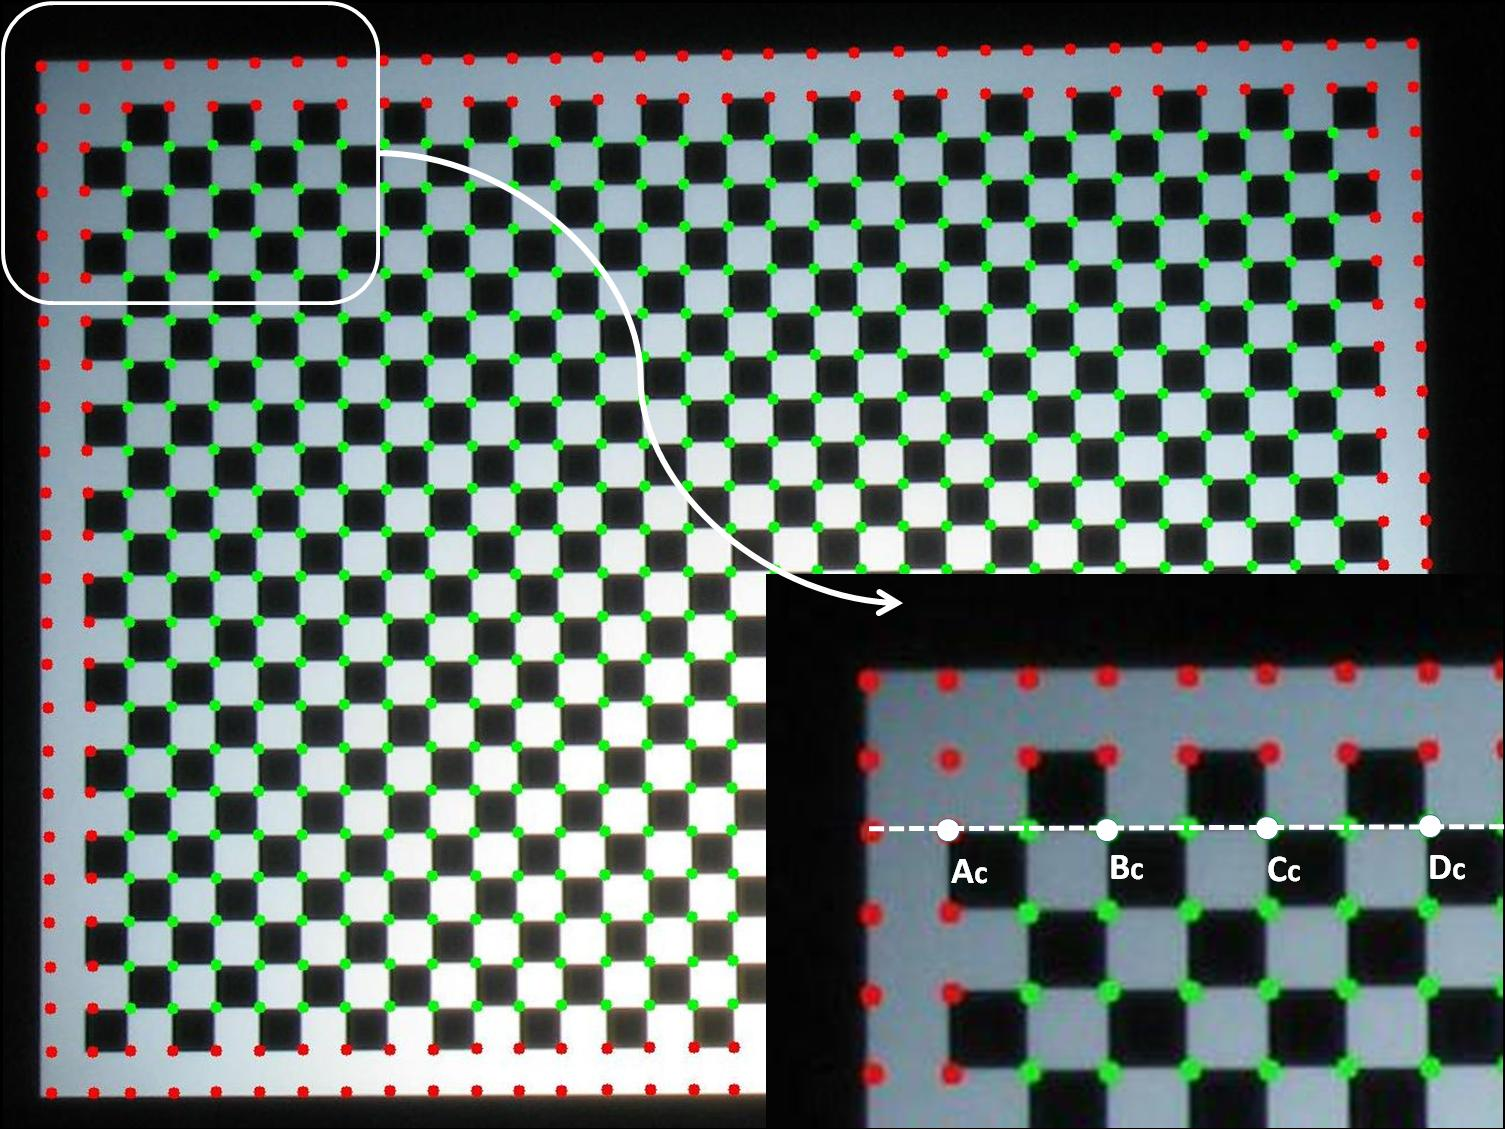
\includegraphics[width=6cm,height=5cm]{figures/cross_rat_img.jpg} 
\caption{Recovering $A_c$ using $B_c$,$C_c$,$D_c$}
\label{cross_rat_img}
\end{figure}



\subsection{Algorithm}
Process of geometric alignment is partitioned into two major steps: \textit{feature detection and regularization} and \textit{warp map computation}.\newline
1) Feature detection and regularization: It is used for recording the distortion of reference pattern for each projector. Steps are discussed below:
\begin{enumerate}
\item Camera captures the checkerboard pattern projected by each projector.
\item Standard OpenCV algorithm \cite{opencv} is used for detecting inner checkerboard corners(\textit{green} points in figure \ref{cross_rat_img}).
\item Since collinearity is invariant under projective transformation, features collinear in projector image must be 		      collinear in camera space also. In order to account for this, detected locations of features in camera image are regularized by explicitly enforcing collinearity constraint. Specifically, each feature is computed as intersection of vertical and horizontal fitted lines. Figure \ref{linefit_img} shows the difference between raw corner detection(figure \ref{linefit_img}.(a)) and improvements after applying collinearity constraint(figure \ref{linefit_img}.(b)).

\begin{figure}
\centering
\def\tabularxcolumn#1{m{#1}}
\begin{tabularx}{\linewidth}{@{}cXX@{}}
\begin{tabular}{c}
\subfloat[]{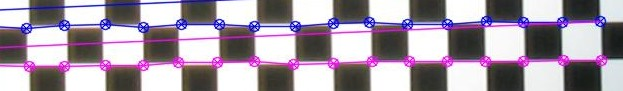
\includegraphics[width=7.5cm,height=1.5cm]{figures/test.jpg}} \\ 
\subfloat[]{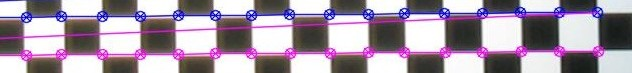
\includegraphics[width=7.5cm,height=1.5cm]{figures/test2.jpg}} \\
\end{tabular}
\end{tabularx}
\caption{Enforcing collinearity constraint in camera-space}
\label{linefit_img}
\end{figure}


\item Once the features are regularized, lost projection region at the boundary are recovered by determining position of \textit{virtual} points(\textit{red} points in figure \ref{cross_rat_img}) using cross-ratio constraint(equation \ref{cross_rat_eqn}).
\item Estimated coordinates for these \textit{virtual} points are further modified by enforcing the collinearity constraint.
\end{enumerate}
2) Warping map computation: This step computes the distortion map(or, the \textit{warp map}) which is used for modifying the image in projector frame buffer such that when projected it retains geometric continuity of the content. This distortion information is extracted from the features detected earlier. Steps for warp-map computation are discussed below:
\begin{enumerate}	     
\item Camera-to-screen homography\cite{elan} is determined to map all subsequent computations to screen space. This step ensures that the final rendered content on the screen will be free from the perspective distortions which get introduced when performing geometric alignment computations entirely in the camera-space.
\item Bounding boxes are computed for each projection region in the screen-space. A bounding box is the convex hull enclosing all features of a projector recovered in feature detection and regularization phase. Figure \ref{all_bboxes} shows the bounding box for the top-left projector in our display arrangement, for rest of the projectors only bounding boxes are highlighted for the sake of clarity. It should be noted that the bounding box of top left projector has covered its entire projection region because we determined the position of \textit{virtual} points as well. 

\begin{figure}
\centering
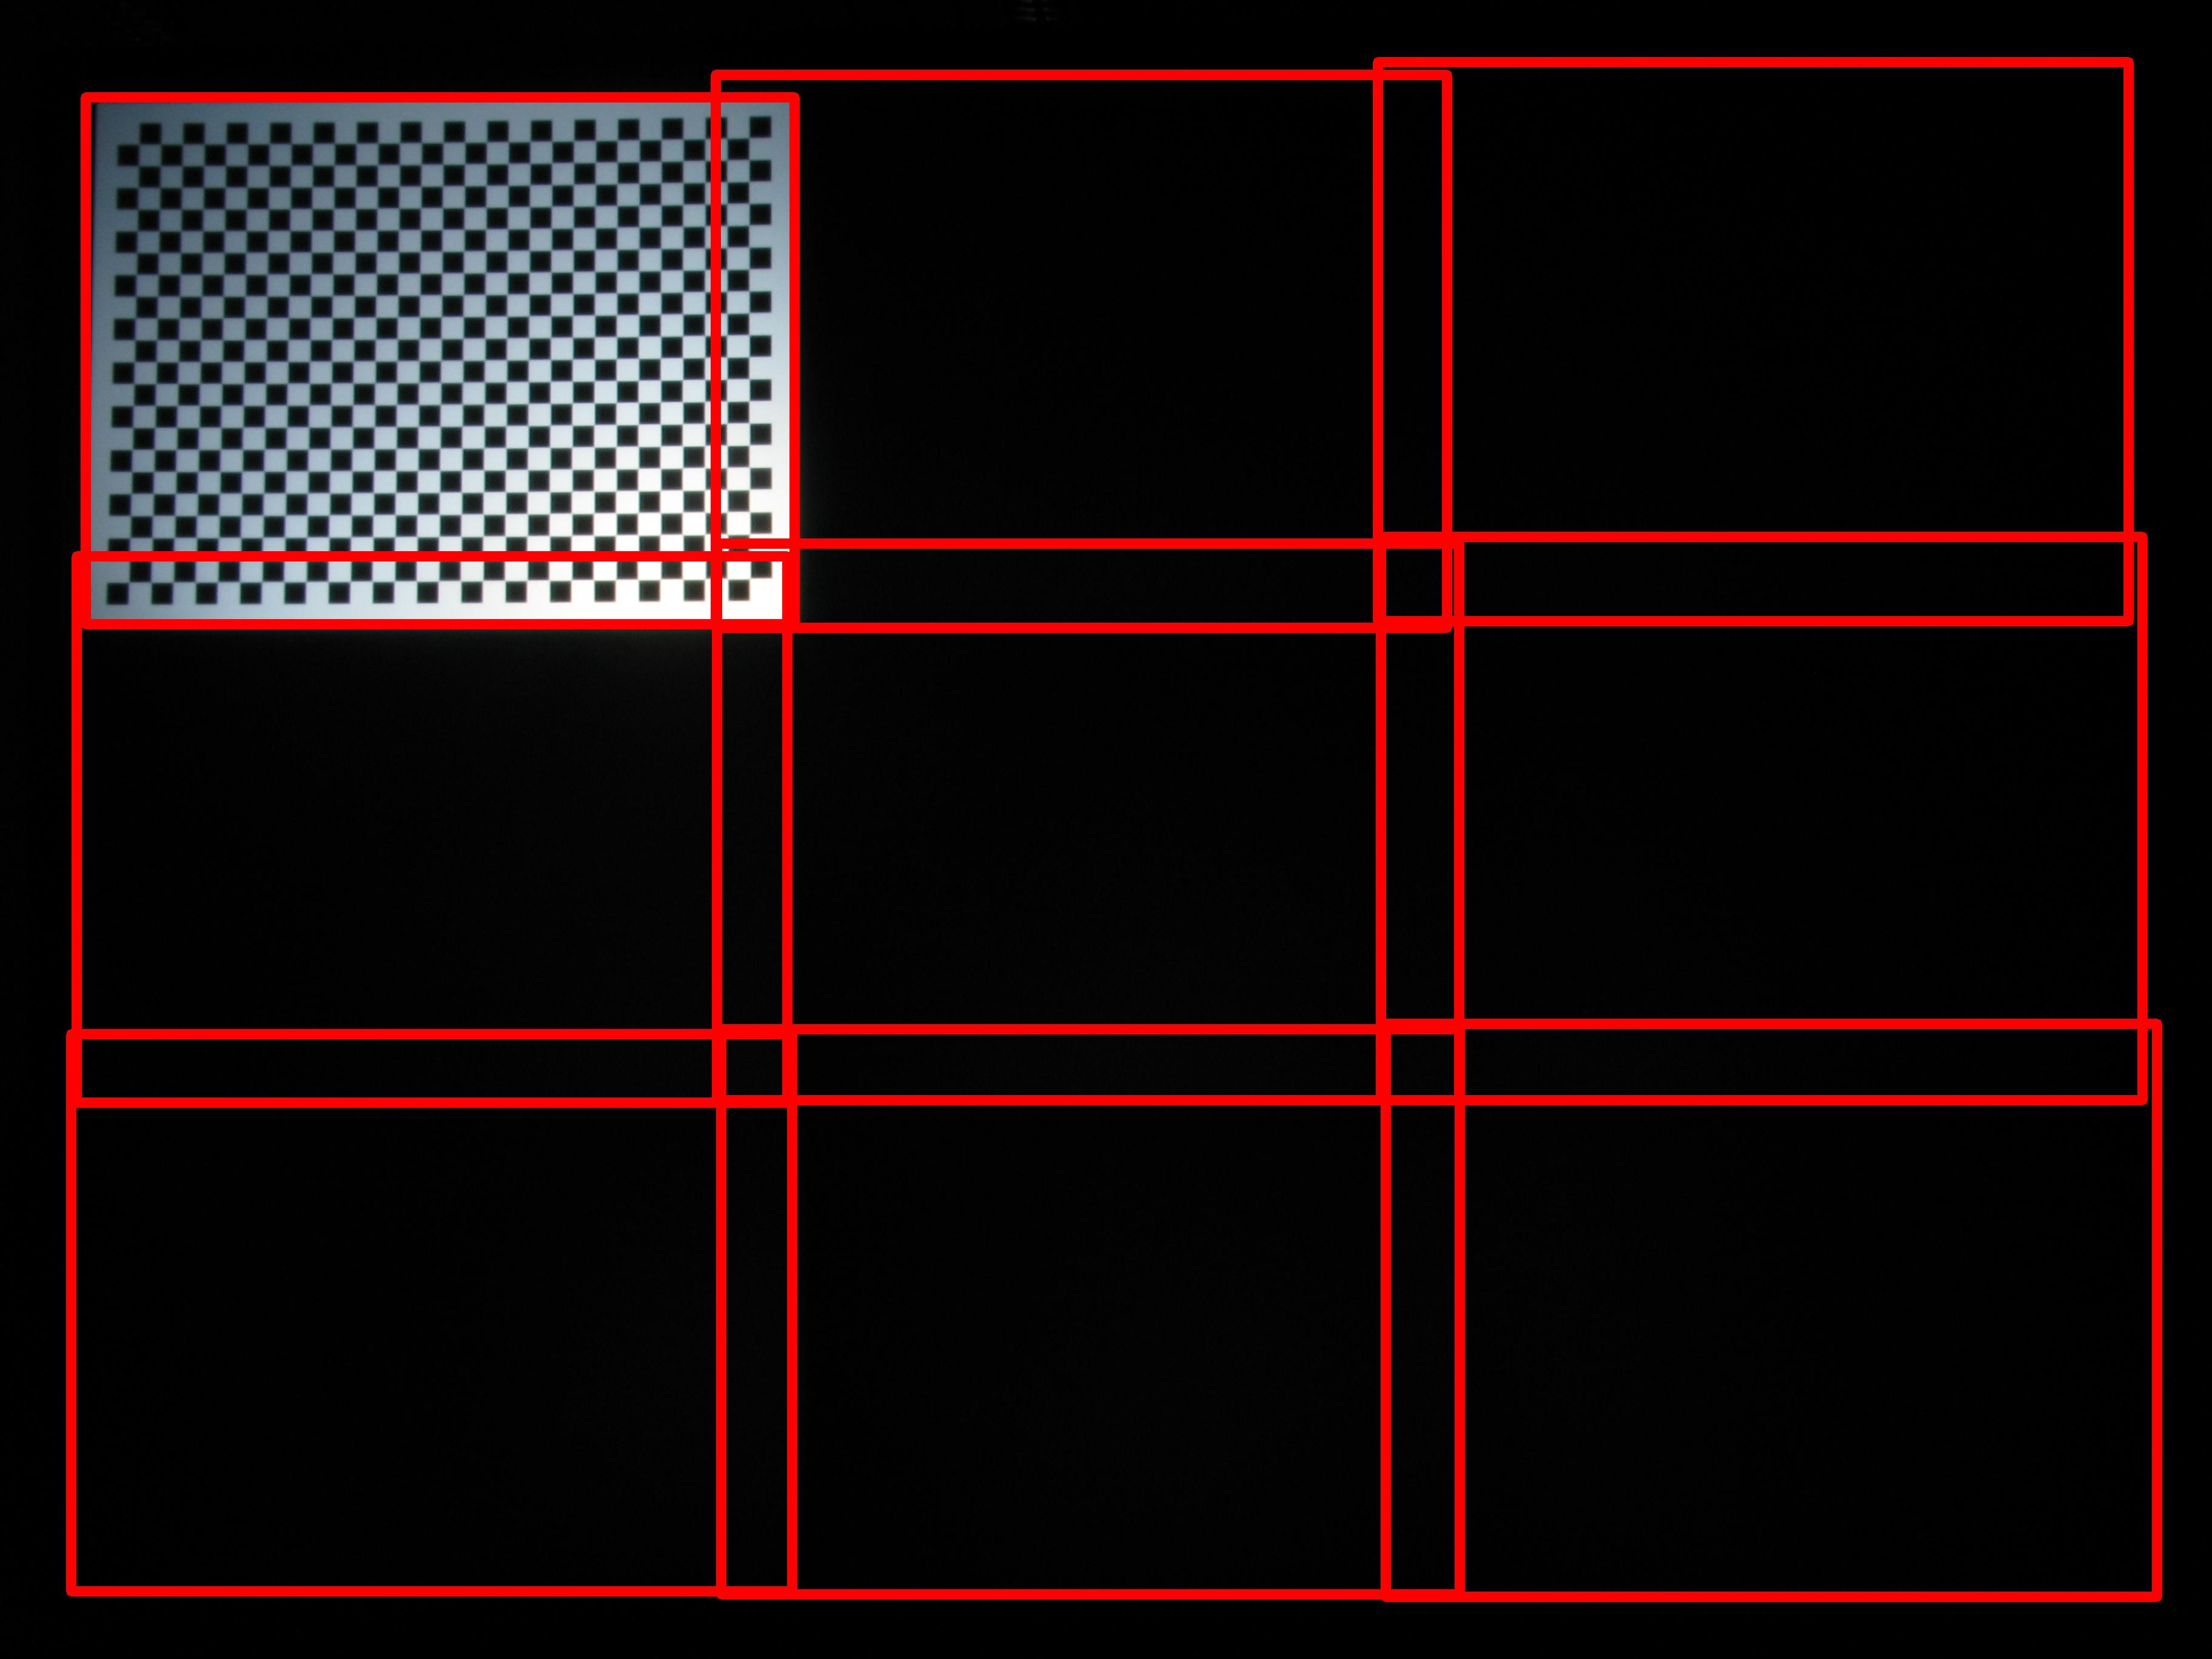
\includegraphics[width=6cm,height=4cm]{figures/all_bboxes.jpg}
\caption{Bounding boxes for all projectors}
\label{all_bboxes}
\end{figure}


\item  A \textit{maximal} box is computed which can contain any local bounding box. Naturally, it corresponds to the box having maximum width and height among that of all local bounding boxes. All local bounding boxes are modified to have maximum width and height.

\item These width and height are equated with width and height of individual projector frame buffers to maintain uniform pixel size regardless of different sizes of projection regions of the projectors on the screen. 

\item A global bounding box is computed which is the convex hull enclosing all local bounding boxes. This global bounding box acts like a global tile coordinate system containing all local bounding boxes(or tiles) and hence all the detected features. This determines the final \textit{tile configuration}.

\item All detected features are mapped to global tile coordinate system to be used for deriving \textit{warp map} information.
\end{enumerate}


\section{Edge blending}
Edge blending algorithm utilizes the projector-overlap information acquired during geometric alignment phase for attenuating the projector image intensity in the overlap regions.
\subsection{Algorithm}
Projector image intensity is attenuated in the overlap region by scaling the pixel values using \textit{alpha map}. An alpha map is a 2D array with one value(called \textit{alpha weight}) for each projector pixel. Steps for edge blending are discussed below:
\begin{enumerate}
\item For each projector, the coordinates of detected feature relative to the global bounding box are computed. It maps the points from camera coordinate system to global bounding box coordinate system. 
\item A \textit{tightest} polygon bounding the detected features for each projector is determined.
\item Each pixel $(x_g,y_g)$ in the global bounding box(or global coordinate frame) is tagged with the index of projectors sharing it.
\item For each projector $p$, \textit{alpha weight} is computed at each pixel $(x_p,y_p)$ using \textit{distance transform} as:

\begin{equation}
\alpha(p,x_p,y_p)=\frac{d_p(x_p,y_p)}{\sum\nolimits_{i \in shares(i,x_g,y_g)} d_i(x_i,y_i)}
\end{equation}
where, $(x_g,y_g)$ are global frame coordinates for pixel $(x_p,y_p)$ in projector $p$ and for pixel $(x_i,y_i)$ in projector(s) $i$, $d_p(x_p,y_p)$(and similarly $d_i(x_i,y_i)$) represents the perpendicular distance of the \textit{closest} boundary of projection region of projector $p$(and similarly projector(s) $i$) from pixel $(x_p,y_p)$(similarly, $(x_i,y_i)$), proposition $shares(i)$ is \textit{true} for any projector $i$ which shares pixel $(x_g,y_g)$ in the global coordinate frame,

\item In order to account for non-linearities in projector's output response, an additional factor \textit{gamma}\cite{paul} is applied to alpha weights as:
\begin{equation}
\alpha(p,x_p,y_p)_\gamma=\alpha(p,x_p,y_p)^{\frac{1}{\gamma(p(x_p,y_p))}}
\end{equation}
where, $\alpha(p,x_p,y_p)$, $\gamma(p(x_p,y_p))$ and  $\alpha(p,x_p,y_p)_\gamma$ represent the alpha weight, gamma value and gamma corrected alpha weight for projector $p$ at pixel $(x_p,y_p)$ respectively.
\end{enumerate}

\section{Practical implementation}
In this section, we give brief details about the hardware setup and software implementation of our multiprojector display system.

\subsection{Hardware}
The seamless display has been achieved by using 120" rear projection screen and arranging the 9 commodity DLP projectors in 3x3 matrix form. The projectors are arranged such that each projector projects an image of more than 40" from the rear. The 9 projected images of projectors are overlapped at the edges and collectively cover the entire screen. The display has aspect ratio of 4:3, screen dimensions of 8' x 6' and the resolution of 7 mega pixels. The display is driven by a cluster of 3 graphics workstations. Each 
graphics workstation drives 3 projectors through 3 graphics cards. 

\subsection{Software}
We use open source software - Chromium and DMX as a software environment to realize the 3x3 projector based seamless display. We use Chromium for running OpenGL based graphics applications and DMX for running other X based desktop applications on the seamless display. We use TiledRenderer\cite{pritam} - an in house MPI based parallel rendering software for viewing the high resolution scientific visualization movies or images. We have customized Chromium , DMX and TiledRenderer to use the warp maps and alpha maps generated by the above algorithm to pre-warp and blend the images to be displayed by individual projectors.


\section{Results}
On our test setup $\sim9.6\%$ more projection region was utilized using our approach. Further, our approach allows for more inter-projector overlap leading to more realistic alpha maps as can be compared in figures \ref{without_crossrat} and \ref{with_crossrat}. Consequently, boundaries are more visible in figure \ref{without_crossrat} as compared to those in figure \ref{with_crossrat}. To quantify geometric alignment accuracy of our system we projected a grid on the display with a resolution of 200 cells per unit area and measured the misalignment at the junctions between adjacent projectors. We found that the average misalignment error for our system was about:$\sim1mm$. 

\begin{figure}
\centering
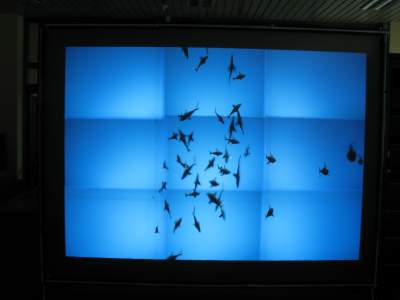
\includegraphics[width=6cm,height=4cm]{figures/without_cross_rat1.jpg}
\caption{Projection using Brown's\cite{brown} approach}
\label{without_crossrat}
\end{figure}


\begin{figure}
\centering
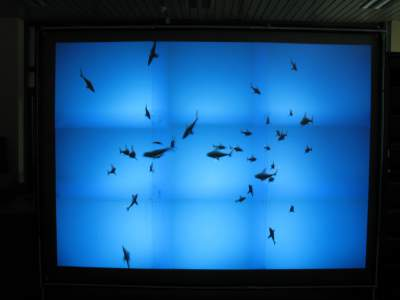
\includegraphics[width=6cm,height=4cm]{figures/with_cross_rat1.jpg}
\caption{Projection using our approach utilizing \textit{cross-ratio} constraint}
\label{with_crossrat}
\end{figure}

\section{Conclusion}
We have described an enhanced multiprojector geometric alignment utilizing \textit{Cross-ratio} invariance based projection region recovery. Brown's method puts a constraint in which atleast outer features of adjacent projector must overlap in order to get geometrically continuous image on the screen. This actually limits their claimed merit of casual alignment of projector. Further, there was no provision for using projection region beyond outermost features. Our approach allows for recovery of artificial feature points at the boundary of each projector's projection region due to which full projection region can be utilized and there is no constraint on projector positioning. Further, utilizing full projection region of each projector increases the area of overlap between adjacent projectors resulting in more uniform edge blending.


\begin{thebibliography}{1}
\bibitem{brown} 
Brown, M.S.; Seales, W.B., ``A practical and flexible tiled display system,'' Computer Graphics and Applications, 2002. Proceedings. 10th Pacific Conference on , vol., no., pp.194,203, 2002


\bibitem{bose}
Bose, S. K.; Sarode, D.M.; Venkata, P.P.K.; Shete, P.P.; Apte, A. G., "High End Scientific Visualization with Scalable Display System," Advances in Computer Engineering (ACE), 2010 International Conference on , vol., no., pp.316,318, 20-21 June 2010

\bibitem{harish}
Nirnimesh; Harish, P.; Narayanan, P. J., "Garuda: A Scalable Tiled Display Wall Using Commodity PCs," Visualization and Computer Graphics, IEEE Transactions on , vol.13, no.5, pp.864,877, Sept.-Oct. 2007

\bibitem{opencv}
Bradski, Dr. Gary Rost and Kaehler, Adrian, "Learning Opencv", 1st Edition, 2008, O'Reilly Media, Inc.



\bibitem{judson}
Hereld, M.; Judson, I.R.; Stevens, R.L., "Introduction to building projection-based tiled display systems," Computer Graphics and Applications, IEEE , vol.20, no.4, pp.22,28, July-Aug. 2000

\bibitem{raskar}
Raskar, R.; Brown, M.S.; Ruigang Yang; Wei-Chao Chen; Welch, G.; Towles, H.; Scales, B.; Fuchs, H., "Multi-projector displays using camera-based registration," Visualization '99. Proceedings , vol., no., pp.161,522, 29-29 Oct. 1999

\bibitem{majum} 
Brown, M.; Majumder, A.; Ruigang Yang, ``Camera-based calibration techniques for seamless multiprojector displays,'' Visualization and Computer Graphics, IEEE Transactions on , vol.11, no.2, pp.193,206, March-April 2005


\bibitem{elan}
Dubrofsky, Elan. "Homography estimation." PhD diss., UNIVERSITY OF BRITISH COLUMBIA, 2009.

\bibitem{greg}
Greg Humphreys, Mike Houston, Ren Ng, Randall Frank, Sean Ahern, Peter D. Kirchner, and James T. Klosowski. 2002. Chromium: a stream-processing framework for interactive rendering on clusters. ACM Trans. Graph. 21, 3 (July 2002), 693-702. 

\bibitem{pritam}
"TiledRenderer - an Object Oriented Framework for MPI Based Parallel 
Rendering", Pritam Prakash Shete, Venkata P P K, Dinesh Sarode, Mohini 
Laghate, Surojit Bose,/Second International Conference on Parallel 
Distributed and Grid Computing (PDGC -2012), Shimla, India/, [2012]

\bibitem{hartley}
Hartley, R.I. and Zisserman, A.,"Multiple View Geometry in Computer Vision", Second edition, 2004, Cambridge University Press

\bibitem{paul}
Edge blending using commodity projectors\newline
\url{http://paulbourke.net/texture_colour/edgeblend/}

\end{thebibliography}
\end{document}
